\documentclass[11pt,fancychapters]{report}
\usepackage[a4paper, total={6in, 8in}]{geometry}
\usepackage{listings}
\usepackage{color}
\usepackage{setspace}
\usepackage{hyperref}
\usepackage{acro}
\usepackage{amsmath}
\usepackage{amsthm}
\usepackage{amsfonts}
\usepackage{graphicx}
\usepackage{geometry}
\usepackage{subcaption}
\usepackage{cancel}
\usepackage{tikz}
\usepackage{color}
\usetikzlibrary{calc,trees,positioning,arrows,chains,shapes.geometric,%
    decorations.pathreplacing,decorations.pathmorphing,shapes,%
    matrix,shapes.symbols}
\DeclareAcronym{etf}{
	short = ETF,
    long = Exchange-Traded Fund,
    class = abbrev
}

\DeclareAcronym{aum}{
	short = AUM,
    long = Assets Under Management,
    class = abbrev
}

\DeclareAcronym{sr}{
	short = SR,
    long = Sharpe Ratio,
    class = abbrev
}

\DeclareAcronym{nyse}{
	short = NYSE,
    long = New York Stock Exchange,
    class = abbrev
}

\DeclareAcronym{hft}{
	short = HFT,
    long = High Frequency Trading,
    class = abbrev
}

\DeclareAcronym{pv}{
	short = PV,
    long = present value,
    class = abbrev
}

\DeclareAcronym{fv}{
	short = FV,
    long = future value,
    class = abbrev
}

\DeclareAcronym{ir}{
	short = IR,
    long = interest rate,
    class = abbrev
}

\DeclareAcronym{capm}{
	short = CAPM,
    long = Capital Assets Pricing Model,
    class = abbrev
}

\DeclareAcronym{apt}{
	short = APT,
    long = Arbitrage Pricing Theory,
    class = abbrev
}

\DeclareAcronym{sma}{
	short = SMA,
    long = simple moving average,
    class = abbrev
}

\DeclareAcronym{mvo}{
	short = MVO,
    long = mean variance optimization,
    class = abbrev
}

\DeclareAcronym{rmse}{
	short = RMSE,
    long = root mean square error,
    class = abbrev
}

\DeclareAcronym{kNN}{
	short = kNN,
    long = k-nearest neighbor,
    class = abbrev
}
\geometry{top=1.3in,bottom=1.3in}
\hypersetup{
    colorlinks,
    citecolor=black,
    filecolor=black,
    linkcolor=black,
    urlcolor=black
}

\definecolor{DarkerGreen}{RGB}{0,179,45}

\definecolor{Code}{rgb}{0,0,0}
\definecolor{Decorators}{rgb}{0.5,0.5,0.5}
\definecolor{Numbers}{rgb}{0.5,0,0}
\definecolor{MatchingBrackets}{rgb}{0.25,0.5,0.5}
\definecolor{Keywords}{rgb}{0,0,1}
\definecolor{self}{rgb}{0,0,0}
\definecolor{Strings}{rgb}{0,0.63,0}
\definecolor{Comments}{rgb}{0,0.63,1}
\definecolor{Backquotes}{rgb}{0,0,0}
\definecolor{Classname}{rgb}{0,0,0}
\definecolor{FunctionName}{rgb}{0,0,.7}
\definecolor{Operators}{rgb}{0,0,0}
\definecolor{Background}{rgb}{0.98,0.98,0.98}

\lstdefinestyle{python}{
  numbers=left,
  numberstyle=\footnotesize,
  numbersep=1em,
  xleftmargin=1em,
  framextopmargin=2em,
  framexbottommargin=2em,
  showspaces=false,
  showtabs=false,
  showstringspaces=false,
  frame=l,
  tabsize=4,
  % Basic
  basicstyle=\ttfamily\small\setstretch{1},
  backgroundcolor=\color{Background},
  language=Python,
  % Comments
  commentstyle=\color{Comments}\slshape,
  % Strings
  stringstyle=\color{Strings},
  morecomment=[s][\color{Strings}]{"""}{"""},
  morecomment=[s][\color{Strings}]{'''}{'''},
  % keywords
  morekeywords={import,from,class,def,for,while,if,is,in,elif,else,not,and,or,print,break,continue,return,True,False,None,access,as,,del,except,exec,finally,global,import,lambda,pass,print,raise,try,assert},
  keywordstyle={\color{Keywords}\bfseries},
  % additional keywords
  morekeywords={[2]@invariant},
  keywordstyle={[2]\color{Decorators}\slshape},
  emph={self},
  emphstyle={\color{self}\slshape},
  breaklines=true
}

\newtheorem{exmp}{Example}[section]

\newcommand{\codeExample}[2]{
	\begin{exmp}
      #1
      \noindent\begin{minipage}{\linewidth}
      \begin{lstlisting}[style=python]
          #2
      \end{lstlisting}
      \end{minipage}
    \end{exmp}
}

\newcommand\MyLBrace[2]{%
  \left.\rule{0pt}{#1}\right\}\text{#2}}
  
\tikzset{
>=stealth',
  punktchain/.style={
    rectangle, 
    rounded corners, 
    % fill=black!10,
    draw=black, very thick,
    text width=10em, 
    minimum height=3em, 
    text centered, 
    on chain},
  line/.style={draw, thick, <-},
  element/.style={
    tape,
    top color=white,
    bottom color=blue!50!black!60!,
    minimum width=8em,
    draw=blue!40!black!90, very thick,
    text width=10em, 
    minimum height=3.5em, 
    text centered, 
    on chain},
  every join/.style={->, thick,shorten >=1pt},
  decoration={brace},
  tuborg/.style={decorate},
  tubnode/.style={midway, right=2pt},
}

\title{Compiled Notes}
\author{Joseph Marino}

\begin{document}

\maketitle
\pagenumbering{gobble}
\newpage
\pagenumbering{roman}
\tableofcontents
\newpage
\pagenumbering{arabic}

\chapter{Intelligence}

\section{Intelligence}

Intelligence is a vaguely defined concept. In many situations, we often use the term to refer to the ability to perceive and understand certain concepts, such as math, art, politics, business, etc. But this narrow definition is human specific and fails to capture the broad spectrum that intelligence occupies. Instead, I use this working definition:

\begin{center}
	\textbf{Intelligence} is the ability of a system to perform meaningful actions within a particular environment.
\end{center}

We could argue whether a system that can perceive aspects of its environment but is unable to act is intelligent, but this is meaningless, as this system has no practical purpose. This definition has a few components: A \textbf{system} is some collection of matter: a molecular structure, single-celled organism, animal, machine, computer, human, society, etc. \textbf{Meaningful actions} are more difficult to define. In general terms, these are some non-random interactions with the environment, i.e. the distribution of actions given the environmental state has a relatively low entropy. Often we also associate these actions with achieving some goal or reward, although this is not strictly necessary. Finally, \textbf{within a particular environment} emphasizes the idea that intelligence is always specific to an environment (the data). Intelligence is not a characteristic of a system alone, it's always conditioned on the environment.

\section{Creating Intelligence}

There are two ways in which to create an intelligent system: through \textbf{design} and through \textbf{learning}. In design, one intelligent system constructs another intelligent system. In learning, a system gains intelligence through interaction with the environment.
\chapter{Probability \& Statistics}

Why define a system in terms of probability? Probability allows us to estimating uncertainty arising from stochasticity
\begin{itemize}
    \item in the system itself,
    \item in the measurement process, potentially the result of incomplete observability,
    \item due to limitations in the model, such as discretization.
\end{itemize}
There are two main interpretations of probability. The \textbf{frequentist} approach considers probabilities as the \textit{frequency} of events occurring, calculated over past trials. The \textbf{Bayesian} approach considers probabilities as a specifying the \textit{uncertainty} of events. Under the Bayesian interpretation, probability is a subjective belief, whereas under the frequentist interpretation, probability is an objective frequency of occurring events. While the basic rules of probability are consistent in both approaches, the advantage of the Bayesian approach is that it allows one to model uncertainty even when past trials have not necessarily been observed, providing flexibility. By expressing probability in terms of uncertainty, the Bayesian approach is also deeply connected to information theory (Chapter \ref{chap: information theory}), bringing additional mathematical tools for analysis. 

While probability gives us the tools to account for uncertainty in our estimates, it also brings a separate set of challenges associated with estimating various quantities. Rather than maintaining a single hypothesis about a quantity, probability often requires us to evaluate \textit{all} hypotheses. Instead of ``point estimates," we work with entire ``distributions." This creates computational difficulties stemming primarily from marginalization, i.e. summing or integrating over possible values. One common strategy for dealing with this is to forgo analytical estimates in favor of sampling-based estimates. In Chapter \ref{chap: variational inference}, we discuss variational inference, another technique for overcoming some of these issues.


\section{Probability}

Probabilities are defined for \textbf{random variables}, which can take either \textit{discrete} or \textit{continuous} values. A discrete variable could be whether or not a light switch is on, and a continuous variable could be the level of a light dimmer. A random variable only defines possible values that can be taken; to define the likelihood of the random variable taking each of the values, we must use a \textbf{probability distribution}. In the cases of the discrete and continuous random variables, the total probability of all values must sum to $1$ because the variable must take some value. The light switch must be on or off, and the light dimmer must be at some particular level. To accommodate this requirement, probabilities over discrete and continuous random variables must be handled differently, e.g. replacing summations with integrals, but the underlying rules of probability are identical in both cases.

\subsection{Discrete Random Variables}

Discrete random variables can take a finite or countably infinite number of values. Note that these values may not necessarily be numerical. In describing the probability over the values of a discrete random variable, we use a \textbf{probability mass function (PMF)}. A PMF, $P(x)$, is a function that maps discrete values of a random variable, $x$, to probabilities between $0$ and $1$, i.e.
$$\forall x, 0 \leq P(x) \leq 1. $$
Following our requirement that probability distributions must sum to $1$, we must ensure that
$$ \sum_x P(x) = 1. $$
We refer to a function meeting this requirement as being \textbf{normalized}. 

\subsection{Continuous Random Variables}

Continuous random variables take an uncountably infinite number of values, associated with a real value over some domain. To define the probability over this domain, we use a \textbf{probability density function (PDF)}. Unlike a PMF, a PDF, $p(x)$, is only required to be non-negative:
$$ \forall x, 0 \leq p(x). $$
Again, we must ensure that the total probability sums to $1$. Since we are dealing with a continuous domain, we must integrate:
$$ \int p(x) dx = 1. $$
Again, such a function is considered to be normalized. Note that $p(x)$ does not give the \textit{probability} of the value $x$, but rather, the probability \textit{density} at that point. In other words, with continuous random variables, we can only evaluate the probability of values in terms of intervals. In an infinitesimal interval, $\delta x$, around a point $x$, the probability is $p(x) \delta x$. More generally, we can quantify the probability mass within an interval $[a, b]$ as
$$P_{[a,b]} = \int_a^b p(x) dx. $$
In correspondence with physics, we can evaluate the probability \textit{mass} within an interval, i.e. \textit{volume}, by integrating the probability \textit{density} over that volume. This can also be accomplished by using the \textbf{cumulative density function (CDF)}, which is defined as
$$ \textrm{CDF}(x^\prime) \equiv \int_{- \infty}^{x^\prime} p(x) dx. $$
This allows us to quickly evaluate the probability within an interval as
$$ P_{[a,b]} = \textrm{CDF}(b) - \textrm{CDF}(a). $$

\subsection{Definitions and Rules}

The \textbf{joint distribution} defines the probability of events \textit{jointly} occurring over multiple variables. For instance, with variables $A$ and $B$, the joint distribution $p(A=a,B=b)$ defines the probability that variable $A$ takes the value $a$ \textit{and} variable $B$ takes the value $b$. The joint distribution can decomposed as
\begin{equation}
    p(A,B) = p(A|B)p(B) = p(B|A)p(A).
    \label{eq: def of joint prob}
\end{equation}
This decomposition is known as the \textbf{chain rule of probability}, and can be used to split any joint distribution into a series of \textbf{conditional} and \textbf{marginal distributions}. The conditional distribution defines the probability of an event in one variable occurring \textit{conditioned} on another event occurred in a different variable. Thus, $p(A=a | B=b)$ quantifies the probability that $A$ takes the value $a$ \textit{given} that $B$ takes the value $b$. Intuitively, this is defined as the probability of observing $a$ and $b$ together, divided by the probability of observing $b$ in general:
\begin{equation}
    p(A|B) = \frac{p(A,B)}{p(B)}.
    \label{eq: def of cond prob}
\end{equation}
The denominator here is the marginal distribution, which is obtained from the joint distribution over the variables by \textit{marginalizing}, i.e. summing, over the values of the other variables. To obtain the marginal $p(A)$, we marginalize over the variable $B$:
\begin{equation}
    p(A) = \sum_b p(A, B=b) = \sum_b p(A | B=b) p(B=b).
    \label{eq: def of marginal prob}
\end{equation}
From eq. \ref{eq: def of joint prob}, we can also jump directly to \textbf{Bayes' Rule}, which specifies one conditional probability, e.g. $p(A|B)$, in terms of the other conditional probability and the marginal distributions:
\begin{equation}
    p(A|B) = \frac{p(B|A)p(A)}{p(B)}.
    \label{eq: bayes rule}
\end{equation}

\section{Common Distributions}

\subsection{Probability Mass Functions}


\subsection{Probability Density Functions}


\subsection{Implicitly-Defined Distributions}

Up until now, we have discussed probability distributions that have a well-defined analytical form. These are sometimes referred to as \textit{explicitly-defined} distributions, because the form can be written down explicitly. However, there are also probability distributions that do not have an analytical form. These distributions are often defined in terms of invertible \cite{dinh2014nice} or non-invertible \cite{goodfellow2014generative} transformations of samples from other, simpler distributions. As the transformed distributions can only be evaluated through their samples, they are referred to as \textit{implicitly-defined} distributions \cite{mohamed2016learning}. In general, these distributions offer greater flexibility over explicitly-defined distributions, however, there are also additional difficulties associated with learning these distributions.
\chapter{Information Theory}

\section{Basic Concepts}

\textbf{Entropy} is a measure of the uncertainty of a random variable. It tends to agree with the notion of information. Let $X$ be a random variable, with alphabet $\mathcal{X}$ and probability mass function $p(x) = \text{Pr} (X = x)$, with $x \in \mathcal{X}$. The entropy of $X$ is defined as

\begin{equation}
	H(X) = - \sum_{x \in \mathcal{X}} p(x) \log p(x).
	\label{eq: entropy_definition}
\end{equation}

\noindent The units of entropy depend on the base of the logarithm. If the base is 2, then the units are in bits. If the base is $e$, then the units are in nats. To convert between different units of entropy, use $H_b (X) = (\log_b a) H_a (X)$. Note that entropy can be interpreted as the expectation of $-\log p(x)$. Also, entropy is non-negative: $H(X) \geq 0$.

The \textbf{joint entropy} of multiple random variables is defined similarly:

\begin{equation}
	H(X, Y) = - \sum_{x \in \mathcal{X}} \sum_{y \in \mathcal{Y}} p(x, y) \log p(x, y)
	\label{eq: joint_entropy_definition}
\end{equation}

\noindent Likewise, the \textbf{conditional entropy} is defined as

\begin{align*}
	H(Y | X) &= \sum_{x \in \mathcal{X}} p(x) H(Y | X = x) \\
		     &= - \sum_{x \in \mathcal{X}} p(x) \sum_{y \in \mathcal{Y}} p(y | x) \log p(y | x) \\
		     &= - \sum_{x \in \mathcal{X}} \sum_{y \in \mathcal{Y}} p(x, y) \log p(y | x).
	\label{eq: conditional_entropy_definition}
\end{align*}

\noindent Note that

\begin{equation}
	H(X, Y) = H(X) + H(Y | X).
\end{equation}

\noindent In words, joint entropy = individual entropy + conditional entropy. This also implies that

\begin{equation}
	H(X, Y | Z) = H(X | Z) + H(Y | X, Z).
\end{equation}

\noindent Because conditional entropy involves the conditional probability, we see that $H(Y | X) \neq H(X | Y)$. However,

\begin{equation}
	H(X) - H(X | Y) = H(Y) - H(Y | X).
\end{equation}

\textbf{Relative entropy} is a measure of the distance between two distributions. Put differently, it is the inefficiency of assuming the distribution of the data is $q(x)$ when the true distribution is $p(x)$. This is also referred to as the \textbf{Kullback-Leibler distance} or \textbf{divergence}.

\begin{equation}
	D_{KL} (p(x) || q(x)) = \sum_{x \in \mathcal{X}} p(x) \log \frac{p(x)}{q(x)} = \mathbb{E}_{x \sim p(x)} \Big[ \log \frac{p(x)}{q(x)} \Big]
	\label{eq: KL_definition}
\end{equation}

\noindent Note that if there is a value $x \in \mathcal{X}$ such that $p(x) > 0$ and $q(x) = 0$, then $D_{KL} = \infty$. KL divergence is non-negative and is only zero when $p(x) = q(x)$. It is not symmetric, so it is not a proper distance measure.

\textbf{Mutual Information} is the amount of information that one random variable contains about another random variable. In other words, it is the reduction in the uncertainty of one random variable due to knowledge of the other. It is expressed as the relative entropy between the joint distribution $p(x, y)$ and the product of the marginals $p(x) p(y)$.

\begin{align*}
	I(X; Y) &= \sum_{x \in \mathcal{X}} \sum_{y \in \mathcal{Y}} p(x, y) \log \frac{p(x, y)}{p(x) p(y)} \\
	           &= D_{KL} (p(x, y) || p(x) p(y)) \\
	           &= \mathbb{E}_{x, y \sim p(x, y)} \Big[ \log \frac{p(x, y}{p(x) p(y)} \Big].
\end{align*}

\noindent This can also be written as

\begin{equation}
	I(X; Y) = H(X) - H(X | Y) = H(Y) - H(Y | X).
\end{equation}

\noindent Thus, \textit{$X$ says as much about $Y$ as $Y$ says about $X$}. In words, mutual information is the amount of information in $X$ minus the amount of information in $X$ after observing $Y$ (and vice versa). This corresponds to the amount of information in $X$ that is explained by $Y$ (and, again, vice versa). If $Y$ perfectly explains $X$, then $H(X | Y) = 0$, so $I(X; Y) = H(X)$. At the other extreme, if $Y$ says nothing about $X$, then $H(X | Y) = H(X)$, so $I(X; Y) = 0$. Also, 

\begin{equation}
	I(X; Y) = H(X) + H(Y) - H(X, Y),
\end{equation}

\noindent and

\begin{equation}
	I(X; X) = H(X) - H(X | X) = H(X).
\end{equation}

\noindent Thus, entropy can be considered as the amount of self-information.

















\chapter{Neuroscience}

\section{Neurons}

\section{Neural Circuits}

\section{Brain Structures}
\chapter{Neural Networks}
\section{Basics}


\subsection{Linear Threshold Units}

\subsection{Multi-Layer Perceptrons}

\subsection{Backpropagation}


\chapter{Graphical Models}

\section{Latent Variable Models}

\subsection{Temporal Latent Variable Models}

We have a sequence of observations $\mathbf{x}_{\leq T}$, which extend over $T$ timesteps. Assume we also have a sequence of latent variables $\mathbf{z}_{\leq T}$. If we assume that time only moves in the forward direction, then with parameters $\theta$, we can write the joint probability of this model as

\begin{equation}
	p_\theta (\mathbf{x}_{\leq T}, \mathbf{z}_{\leq T}) = \prod_{t=1}^T p_\theta (\mathbf{x}_{t} | \mathbf{x}_{< t}, \mathbf{z}_{\leq t}) p_\theta (\mathbf{z}_{t} | \mathbf{x}_{< t}, \mathbf{z}_{< t}).
\end{equation}

\noindent The term $p_\theta (\mathbf{x}_{t} | \mathbf{x}_{< t}, \mathbf{z}_{\leq t})$ is the conditional likelihood or observation model, and the term $p_\theta (\mathbf{z}_{t} | \mathbf{x}_{< t}, \mathbf{z}_{< t})$ is the prior, transition, or dynamics model. The full graphical model is represented in figure \ref{fig: full_temporal_model}. The conditional dependencies show that the computation in this model grows exponentially with the sequence length $T$. Later, we will enforce stricter assumptions on the temporal dependencies to make computation tractable.

\begin{figure}[h]
    \centering
    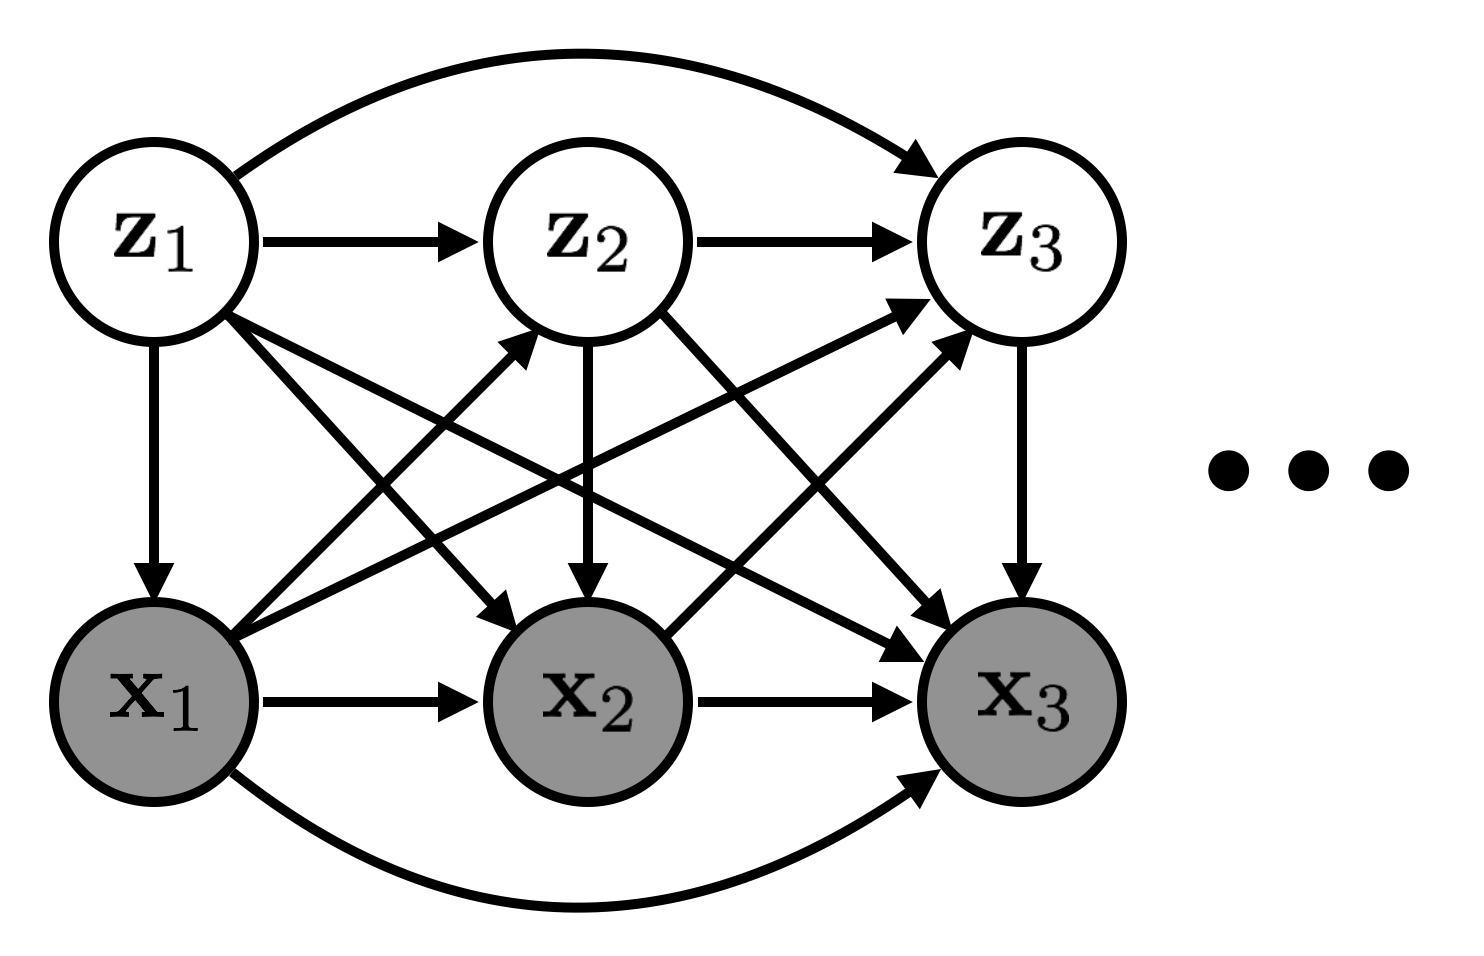
\includegraphics[width=.5\textwidth]{images/graphical_models/full_temporal_model.png}
    \caption{Simplified graphical model representation of temporal latent variable model with all connections present. Note that we're assuming the `arrow of time' points forward; variables can only affect other variables at the current time step or at future time steps. The parameters $\theta$ have been omitted for clarity.}
    \label{fig: full_temporal_model}
\end{figure}

To train or perform inference with this model, we need to compute $p_\theta (\mathbf{x}_{\leq T})$, which involves marginalizing over all states $\mathbf{z}_{\leq T}$:

\begin{equation}
	\log p_\theta (\mathbf{x}_{\leq T}) = \log \int p_\theta (\mathbf{x}_{\leq T}, \mathbf{z}_{\leq T}) d \mathbf{z}_{\leq T}
\end{equation}

\noindent Instead, we'll use an approximate posterior distribution, $q (\mathbf{z}_{\leq T} | \mathbf{x}_{\leq T})$, to compute a lower bound on this quantity:

\begin{equation}
	\log p_\theta (\mathbf{x}_{\leq T}) = \log \mathbb{E}_{q (\mathbf{z}_{\leq T} | \mathbf{x}_{\leq T})} \left[ \frac{p_\theta (\mathbf{x}_{\leq T}, \mathbf{z}_{\leq T})}{q (\mathbf{z}_{\leq T} | \mathbf{x}_{\leq T})} \right]
\end{equation}

\begin{equation}
	\log p_\theta (\mathbf{x}_{\leq T}) \geq \mathbb{E}_{q (\mathbf{z}_{\leq T} | \mathbf{x}_{\leq T})} \left[ p_\theta (\mathbf{x}_{\leq T}, \mathbf{z}_{\leq T}) - q (\mathbf{z}_{\leq T} | \mathbf{x}_{\leq T}) \right]
\end{equation}

\chapter{Representations \& Representation Learning}

\section{Motivation \& Definitions}

Overview of types of representations. How do we learning representations? What training criteria/conditions result in different representations? Are certain representations better than others? In which cases and why? The quality of a representation can only fundamentally be judged by its usefulness in helping to perform some task. That is, representations must be viewed in the context of a task.



\section{Disentangled Representations}

Define disentanglement. Why are disentangled representations helpful? Trade off between disentanglement and faithfully representing the data. How do we learn disentangled representations, while at the same time, respecting the structure of the latent space? Importance of priors.

Two random variables are \textbf{independent} if their joint probability can be expressed as the product of their marginals:

\begin{equation}
	p(\mathbf{x}, \mathbf{y}) = p(\mathbf{x}) p(\mathbf{y}),
\end{equation}

\noindent and they are \textbf{conditionally independent} if their conditional joint probability can be expressed as

\begin{equation}
	p(\mathbf{x}, \mathbf{y} | \mathbf{z}) = p(\mathbf{x} | \mathbf{z}) p(\mathbf{y} | \mathbf{z}).
\end{equation}

Independence is related to covariance, but is a stronger property. Two variables that are independent have zero covariance and two variables that have non-zero covariance are dependent. Zero covariance implies that the variables have no \textit{linear} dependence. Independence implies that the variables also have no \textit{non-linear} dependence. That is, it is possible for two dependent variables to have zero covariance. 
\\
\\
\noindent \textbf{Notes:}

\cite{cheung2014discovering} propose using a cross-covariance penalty term in the setting of semi-supervised learning of the form:

\begin{equation}
	C(\hat{\mathbf{y}}^{1 \dots N}, \mathbf{z}^{1 \dots N}) = \frac{1}{2} \sum_{ij} \left[ \frac{1}{N} \sum_n (\hat{y}^n_i - \bar{\hat{y}}_i) (z^n_j - \bar{z}_j) \right]^2,
\end{equation}

\noindent where $\hat{\mathbf{y}}$ is a vector of (one-hot) inferred labels and $\mathbf{z}$ is a latent representation. $N$ is the batch size.


\cite{higgins2016early} propose to use a regularization weight in a VAE setting to ``upweight" the amount of regularization as a means of promoting \textbf{redundancy reduction and independence} among the latent representation. They also argue for the importance of \textbf{dense sampling of the (continuous) data manifold} for disentanglement. Sparse sampling of the data manifold results in ambiguity is the manifold interpretation, requiring additional supervision for disentanglement.

\cite{siddharth2016inducing} use supervision to impose structure on part of the latent representation in a VAE.

Dropout \cite{srivastava2014dropout} is a technique for preventing ``fragile coadaptation" between units within a representation, effectively enforcing that they represent different (independent) quantities. This technique also results in redundancy within the representation.
\chapter{Predictive Coding}

\section{Introduction}

Predictive coding, in its current form, was formalized by \cite{rao1999predictive}. This theoretical neuroscience model posited that sensory processing is a filtering problem, in which latent states underlying the environmental stimuli are estimated according to their agreement with the observed input as well as prior beliefs about these quantities. This offered an explanation for ``extra-classical" receptive field effects in visual processing, in which stimuli outside the receptive field of a particular cortical neuron are able to affect that neuron's activity. This was explained as the result top-down prior beliefs.

However, the notion of perception as a generative process dates back to at least \cite{von1867handbuch}. \textit{TODO: mention other early work before Rao and Ballard with similar ideas}

Predictive coding claims that sensory processing, i.e. perception, is fundamentally about constructing a generative model of the input sensory signal. To perform \textit{inference} in this model (to perceive), the model uses its current estimate of the latent variables underlying the environment to generate reconstructions or predictions of the input. Using the residual (error) from this reconstruction or prediction, along with residuals from prior beliefs, the model updates its estimate of these latent variables. \textit{Learning} corresponds to updating the parameters of the generative model to improve these overall residuals.
\newline

\subsection{Literature Summary}

\noindent \cite{clark2013whatever} provides a survey of the area of predictive coding
\newline

\noindent \cite{friston2002functional, friston2003learning, friston2005theory} presents a free energy formulation of predictive coding that uses expectation maximization. Primarily focuses on the static setting. Puts forth a theory of cortical processing as carrying out predictive coding.
\newline

\noindent \cite{friston2003dynamic} presents \textit{dynamic causal modeling}.
\newline

\noindent \cite{friston2008variational} presents \textit{variational filtering}.
\newline

\noindent \cite{friston2008DEM} presents \textit{dynamic expectation maximization} (DEM).
\newline

\noindent \cite{friston2010generalised} presents \textit{generalized filtering}, which does not make the mean-field assumption and instead treats all unknown variables as conditionally dependent. This differs from variational filtering \cite{friston2008variational} in that it assumes the parameters and precisions also change with time, with a prior on smoothness of these changes.
\newline

\noindent \cite{feldman2010attention} claims that attention can be formulated as the adjustment of prior precisions in the predictive coding model.
\newline

\noindent \cite{friston2011action}, \cite{friston2013anatomy} , \cite{friston2015active} \cite{friston2016active_process}, \cite{friston2016active} discuss \textit{active inference}.
\newline

\section{The Static Setting}

\subsection{MAP State Estimation in a One--Level Model}

Consider a situation in which the value of a single latent variable $z$ must be inferred from a single observed variable $x$. This is represented by the graphical model in figure  \ref{fig: simple_latent_model}. Let $g$ denote a non-linear function defining how $z$ generates $x$. Assume that the generated output takes the form of a normal distribution with mean $\mu_x = g(z)$ and constant variance $\sigma^2_x$:

\begin{figure}
    \centering
    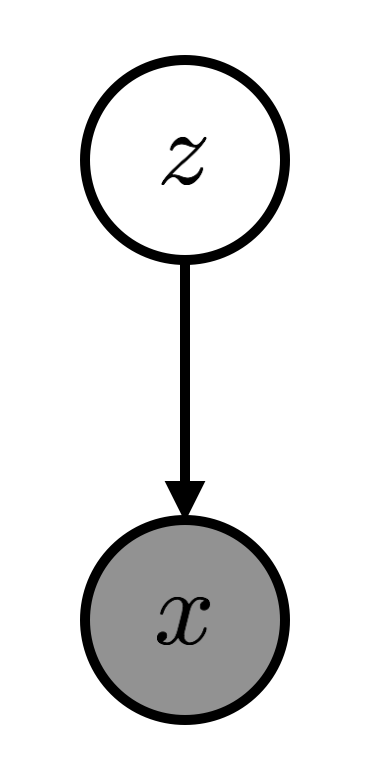
\includegraphics[width=0.15\textwidth]{images/predictive_coding/simple_latent_graphical_model.png}
    \caption{A graphical model denoting a latent variable model in which a single latent variable $z$ generates a single observed variable $x$. In predictive coding, we typically assume that $p(z)$ and $p(x|z)$ are Gaussian densities, and the generative mapping from $z$ to $x$ is a non-linear function.}
    \label{fig: simple_latent_model}
\end{figure}

\begin{equation}
	p (x | z) = \mathcal{N} (x; g(z), \sigma^2_x).
\end{equation}

\noindent Recall that in one dimension, a normal distribution takes the form

\begin{equation}
	\mathcal{N} (x; \mu, \sigma^2) = \frac{1}{\sqrt{2 \pi \sigma^2}} e^{-\frac{(x - \mu)^2}{2 \sigma^2}}.
	\label{eq: 1d gaussian}
\end{equation}

\noindent We will place a prior on $z$, which we also assume is a normal distribution with constant mean $\mu_p$ and constant variance $\sigma^2_p$:

\begin{equation}
	p (z) = \mathcal{N} (z; \mu_p, \sigma^2_p).
\end{equation}

\noindent To infer the posterior distribution of $z$, we can use Bayes' rule to invert the generative model:

\begin{equation}
	p (z | x) = \frac{p(x | z) p(z)}{p(x)},
\end{equation}

\noindent where the marginal distribution in the denominator is given as

\begin{equation}
	p (x) = \int p(x | z) p(z) dz.
	\label{eq: intractable integration}
\end{equation}

In general, computing the exact posterior distribution is computationally intractable due to the integration over $z$ in eq. \ref{eq: intractable integration}. Instead, we'll resort to variational inference\footnote{We are not actually using variational inference here, since the maximum of $p(z | x)$ must also be the maximum of $p(x, z)$ through the definition of conditional probability: $p(z|x) = \frac{p(x, z)}{p(x)}$, since $p(x)$ does not depend on the value of $z$. } to find the maximum (mode) of the posterior, otherwise known as the maximum a posteriori or MAP estimate. This is the \textit{most likely} estimate of the value of $z$. We will define our approximate distribution, a point mass estimate at $\mu_q$, as $q(z|x) = \delta (z = \mu_q)$, with the MAP estimate denoted as $\hat{\mu}_q$.

We want to maximize the evidence lower bound (ELBO), $\mathcal{L}$:

\begin{equation}
	\mathcal{L} = \mathbb{E}_{z \sim q(z|x)} \left[ \log p(x, z) - \log q(z|x) \right] = \mathbb{E}_{z \sim q(z|x)} \left[ \log p(x|z) + \log p(z) - \log q(z|x) \right] 
	\label{eq: elbo 1}
\end{equation}

\begin{equation}
	\mathcal{L} = \log \left( \frac{1}{\sqrt{2 \pi \sigma_x^2}} e^{-\frac{(x - g(\mu_q))^2}{2 \sigma_x^2}} \right) + \log \left( \frac{1}{\sqrt{2 \pi \sigma_p^2}} e^{-\frac{(\mu_q - \mu_p)^2}{2 \sigma_p^2}} \right)
	\label{eq: elbo 2}
\end{equation}

\begin{equation}
	\mathcal{L} = -\frac{1}{2} \log ( 2 \pi \sigma_x^2 )  - \frac{(x - g(\mu_q))^2}{2 \sigma_x^2} - \frac{1}{2} \log ( 2 \pi \sigma_p^2 ) -\frac{(\mu_q - \mu_p)^2}{2 \sigma_p^2}
	\label{eq: elbo 3}
\end{equation}

\begin{equation}
	\mathcal{L} = \frac{1}{2} \left( - \log ( \sigma_x^2 )  - \frac{(x - g(\mu_q))^2}{\sigma_x^2} - \log ( \sigma_p^2 ) -\frac{(\mu_q - \mu_p)^2}{\sigma_p^2} \right) + \text{const.}
	\label{eq: elbo 4}
\end{equation}

\noindent In going from eq. \ref{eq: elbo 1} to eq. \ref{eq: elbo 2}, we used the fact that $q(z|x)$ is a delta function, so the expectation becomes an evaluation at a single point, $z=\mu_q$. The expectation of $q(z|x)$ at this point is $1$, so $\log q(z|x)$ evaluates to $0$. To find the MAP estimate, we must solve the following optimization problem:

\begin{equation}
	\hat{\mu}_q = \text{argmax}_{\mu_q} \mathcal{L} =  \text{argmax}_{\mu_q} \frac{1}{2} \left( - \log ( \sigma_x^2 )  - \frac{(x - g(\mu_q))^2}{\sigma_x^2} - \log ( \sigma_p^2 ) -\frac{(\mu_q - \mu_p)^2}{\sigma_p^2} \right).
\end{equation}

\noindent To use first-order optimization methods, we must find the partial derivative of $\mathcal{L}$ w.r.t. $\mu_q$:

\begin{equation}
	\frac{\partial \mathcal{L}}{\partial \mu_q} = \frac{x - g(\mu_q)}{\sigma_x^2} \frac{d g}{d \mu_q} + \frac{\mu_q - \mu_p}{\sigma_p^2}
	\label{eq: 1d gradient}
\end{equation}

\noindent We see that we have two terms: \textbf{the first term moves the estimate toward agreement with the observation}, and \textbf{the second term moves the estimate toward agreement with the prior}. Each of these terms are weighted by their corresponding variances. In other words, inference (i.e. finding the optimal estimate of $\mu_q$) involves a weighted combination of \textit{bottom-up} and \textit{top-down} information. By repeatedly moving our estimate $\mu_q$ along this gradient, we can hopefully arrive at the MAP estimate $\hat{\mu}_q$. Note that we may not find the true value $\hat{\mu}_q$ if the optimization surface is non-convex. 

We would like to extend this single dimensional model to handle latent and observed variables of arbitrary size. In this setting, $\mathbf{x}$ and $\mathbf{z}$ are now vectors. The conditional likelihood, $p(\mathbf{x} | \mathbf{z}) = \mathcal{N} (\mathbf{x}; \bm{\mu}_\mathbf{x} = g(\mathbf{z}), \bm{\Sigma}_\mathbf{x})$ is now a multi-variate Gaussian distribution. The general form for this distribution is

 \begin{equation}
	\mathcal{N} (\mathbf{x}; \bm{\mu}, \bm{\Sigma}) = \frac{1}{(2 \pi)^{n/2} | \bm{\Sigma}|^{1/2}}  e^{-\frac{1}{2}(\mathbf{x} - \bm{\mu})^\intercal \bm{\Sigma}^{-1}(\mathbf{x} - \bm{\mu})},
	\label{eq: multi-variate gaussian}
\end{equation}

\noindent where $\bm{\Sigma}$ is the covariance matrix, $| \bm{\Sigma}|$ is the determinant of $\bm{\Sigma}$, and $n$ is the dimensionality of the vector $\mathbf{x}$. The prior on $\mathbf{z}$ is also a multi-variate Gaussian: $p(\mathbf{z}) = \mathcal{N} (\mathbf{z}; \bm{\mu}_p, \bm{\Sigma}_p)$. The MAP estimate is now a vector, $\hat{\bm{\mu}}_q$, of the most likely estimate of $\bm{\mu}_q$. To find this estimate, we must again optimize $\mathcal{L}$ w.r.t. $\bm{\mu}_q$. Repeating the steps above, the gradient, $\nabla_{\bm{\mu}_q} \mathcal{L}$, is given as:

\begin{equation}
	\nabla_{\bm{\mu}_q} \mathcal{L} =  \left( \frac{d g}{d \bm{\mu}_q} \right)^\intercal \bm{\Sigma}^{-1}_\mathbf{x} (\mathbf{x} - g(\bm{\mu}_q)) + \bm{\Sigma}^{-1}_p (\bm{\mu}_q - \bm{\mu}_p).
	\label{eq: multi-dimensional gradient}
\end{equation}

\section{The Dynamic Setting}

\section{Attention}

\section{Active Inference}

\section{Neural Implementation}

\subsection{Correspondence with Cortical Mircrocircuits}

\noindent \cite{bastos2012canonical} outlines ideas about correspondence between predictive coding and cortical microcircuits.
\newline

\noindent \cite{kanai2015cerebral} proposes that the pulvinar region of the thalamus is involved in setting precisions of predictions.
\newline

\noindent \cite{bogacz2017tutorial} gives an introductory tutorial to predictive coding with ideas about implementing predictive coding in neocortex.
\newline

\noindent \cite{whittington2017approximation} draws comparisons between backprop and predictive coding.
\newline


\chapter{Programming \& Experimental Practices}

This chapter contains some helpful practices for carrying out (machine learning) research projects.

\section{GitHub}

\href{https://github.com/}{GitHub} is an online platform for project source control. It is essential when collaborating on projects, as it allows you to meticulously track changes and manage conflicts between multiple versions of the code. But GitHub is also helpful when working alone on a project across multiple machines or if you just want to open source your code. The following are the basic commands for using GitHub:
\newline

\noindent \textbf{Clone a repository}:

\begin{lstlisting}[style=python]
git clone <repository address>
\end{lstlisting}

\noindent \textbf{Add a file to the repository}:

\begin{lstlisting}[style=python]
git add <filename>
\end{lstlisting}

\noindent \textbf{Or to add everything to the repository}:

\begin{lstlisting}[style=python]
git add .
\end{lstlisting}

or

\begin{lstlisting}[style=python]
git add -A
\end{lstlisting}

\noindent \textbf{Commit changes to the repository}:

\begin{lstlisting}[style=python]
git commit -m "<message>"
\end{lstlisting}

or

\begin{lstlisting}[style=python]
git commit
\end{lstlisting}

\noindent Note that if you run the second command, you will enter a vi interface where you can enter a multi-line message. To exit, type esc :wq

\noindent \textbf{Push all committed changes to the repository}:

\begin{lstlisting}[style=python]
git push
\end{lstlisting}

\noindent \textbf{Pull the repository}:

\begin{lstlisting}[style=python]
git pull
\end{lstlisting}

\noindent \textbf{To create a new branch}:

\begin{lstlisting}[style=python]
git branch <branch name>
\end{lstlisting}

\noindent \textbf{Switch current branch}:

\begin{lstlisting}[style=python]
git checkout <branch name>
\end{lstlisting}

\noindent \textbf{Merge branch changes back into master (while currently checking out other branch)}:

\begin{lstlisting}[style=python]
git merge master
\end{lstlisting}

\noindent You can send pull requests on GitHub.com. After the branch is merged, you can delete the branch on the website.
\newline

\noindent To conclude, a good workflow practice is to (1) pull the repository at the beginning of each work session, (2) push any incremental changes at regular intervals, and (3) create new branches for any major changes to be implemented.

\section{Logging}

Maintaining proper records of experiments is an essential part of conducting good research. Scientific notebooks (preferably in a digital format) are often helpful for keeping high-level notes about experiments, but one must keep experimental logs to track the different experimental set-ups that have been tested and the results. These are vital for surveying your project (what set-ups work? what set-ups should we consider trying?) and eventually communicating your results. Implementing and keeping track of these logs can seem like a hassle, but they are just as important as the experimental code itself.



\section{Plotting}


\bibliographystyle{apalike}
\bibliography{main}
\appendix
\chapter{Appendix 1} \label{App:AppendixA}

\end{document}